\section{Auswertung}
\label{sec:Auswertung}
\subsection{Runder Stab einseitig eingespannt}
\begin{table}[H]
  \centering
  
  \csvreader[tabular=c|c,
  head=false, 
  table head= Messung & $d\:/\:\si{\milli\meter}$ \\
  \midrule,
  late after line= \\]
  {csvData/Durchmesser.csv}{1=\eins, 2=\zwei}{$\num{\eins}$ & $\num{\zwei}$}
  
  \caption{Durchmesserwerte des runden Stabes}
  \label{tab:a}
\end{table}

Mit den Messwerten aus Tabelle \ref{tab:a} lässt sich
der Durchmesser des runden Stabes mit Hilfe der Formeln
für den Mittelwert

\begin{equation}
  \bar{x}=\frac{1}{n} \cdot \sum_{i=1}^n x_i
  \label{eq:a}
\end{equation}

\noindent und den Standardfehler des Mittelwertes

\begin{equation}
  \Delta\bar{x}=\sqrt{\frac{1}{n(n-1)}\cdot \sum_{i=1}^n(x_i-\bar{x})^2}
  \label{eq:b}
\end{equation}

\noindent als 

\begin{equation*}
  d=(9,980 \pm 0,012)\,\si{\milli\meter}
\end{equation*}

\noindent angeben. Der Radius beträgt somit

\begin{equation*}
  R=(4,990 \pm 0,006)\,\si{\milli\meter}.
\end{equation*}
\noindent Das Flächenträgheitsmoment des runden Stabes kann nach Formel (FLÄCHENTRÄGHEITSMOMENT RUND)
als

\begin{equation*}
  I_{Rund}=(0,003919 \pm 0,000005)\,\si{\meter \tothe{4}}
\end{equation*}

\noindent berechnet werden. 


\begin{table}[H]
  \centering
  
  \csvreader[tabular=c|c|c|c,
  head=false, 
  table head= $x\:/\:\si{\centi\meter}$ & $D_{Ohne Gewicht}\:/\:\si{\milli\meter}$ & $D_{Mit Gewicht}\:/\:\si{\milli\meter}$ & $D_{Differenz}\:/\:\si{\milli\meter}$\\
  \midrule,
  late after line= \\]
  {csvData/tabelle1.csv}{1=\eins, 2=\zwei, 3=\drei, 4=\vier}{$\num{\eins}$ & $\num{\zwei}$ & $\num{\drei}$ & $\num{\vier}$}
  
  \caption{Messwerte des runden Stabes bei einseitiger Einspannung}
  \label{tab:b}
\end{table}

Mit Hilfe einer Linearen Ausgleichsrechnung der Messwerte
aus Tabelle \ref{tab:b} kann der Elastizitätsmodul aus dem 
Faktor $F/2EI_{Rund}$ aus Gleichung (REFERENZ) bestimmt werden, der der Steigung 

\begin{equation*}
  m=(0,0641 \pm 0,0008)\,\si{\meter\tothe{-2}}
\end{equation*}

\noindent der Ausgleichsgeraden
in Abbildung \ref{fig:a} entspricht.

Aus dem Zusammenhang 

\begin{equation}
  E_{Rund}=\frac{F}{2 \cdot m \cdot I_{Rund}}
\end{equation}

\noindent folgt dann, mit dem Wert $F=5,3327\,\si{\newton}$ des verwendeten Gewichtes,

\begin{equation*}
  E=(85,4 \pm 1,1) \cdot 10^{9} \,\si{\kilo\gram\per\meter\per\second\squared}
\end{equation*}

\noindent als Wert für den Elastizitätsmodul. (VERGLEICH MIT LITERATUR)


\begin{figure}[H]
  \centering
  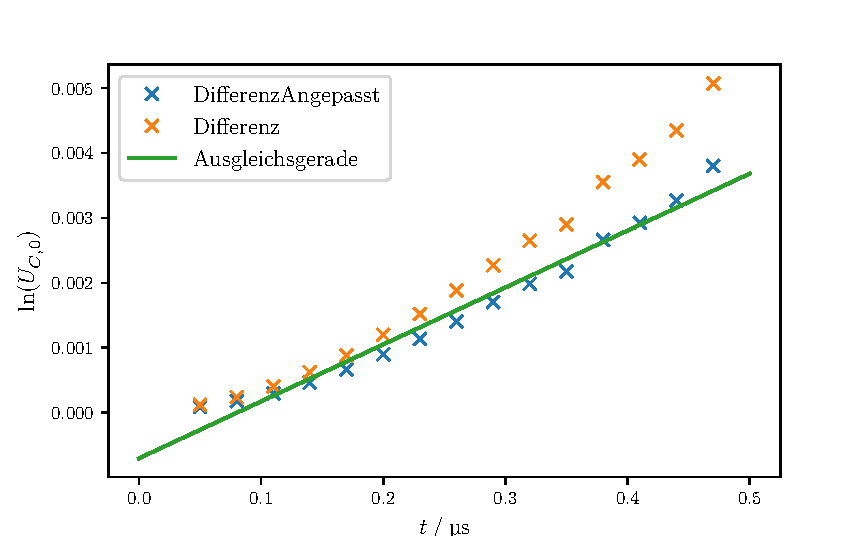
\includegraphics{build/plot1.pdf}
  \caption{Runder Stab einseitig eingespannt}
  \label{fig:a}
\end{figure}



\subsection{Eckiger Stab einseitig eingespannt}

\begin{table}[H]
  \centering
  
  \csvreader[tabular=c|c|c,
  head=false, 
  table head= Messung & $h\:/\:\si{\milli\meter}$ & $b\:/\:\si{\milli\meter}$\\
  \midrule,
  late after line= \\]
  {csvData/Breite.csv}{1=\eins, 2=\zwei, 3=\drei}{$\num{\eins}$ & $\num{\zwei}$ & $\num{\drei}$}
  
  \caption{Höhen- und Breitenwerte des eckigen Stabes}
  \label{tab:c}
\end{table}

Mit den Messwerten aus Tabelle \ref{tab:b} lässt sich
der die Höhe des eckigen Stabes mit Hilfe der Formeln
\ref{eq:a} und \ref{eq:b} als 

\begin{equation*}
  h=(9,960 \pm 0,013)\,\si{\milli\meter}
\end{equation*}
\noindent und die Breite als

\begin{equation*}
  b=(9,995 \pm 0,012)\,\si{\milli\meter}
\end{equation*}

\noindent angeben.Das Flächenträgheitsmoment des eckigen Stabes kann nach Formel (FLÄCHENTRÄGHEITSMOMENT Eckig)
als

\begin{equation*}
  I_{Eckig}=(85,4 \pm 1,1)\cdot 10^{-9}\,\si{\meter \tothe{4}}
\end{equation*}

\noindent berechnet werden. 

\begin{table}[H]
  \centering
  
  \csvreader[tabular=c|c|c|c,
  head=false, 
  table head= $x\:/\:\si{\centi\meter}$ & $D_{Ohne Gewicht}\:/\:\si{\milli\meter}$ & $D_{Mit Gewicht}\:/\:\si{\milli\meter}$ & $D_{Differenz}\:/\:\si{\milli\meter}$\\
  \midrule,
  late after line= \\]
  {csvData/tabelle2.csv}{1=\eins, 2=\zwei, 3=\drei, 4=\vier}{$\num{\eins}$ & $\num{\zwei}$ & $\num{\drei}$ & $\num{\vier}$}
  
  \caption{Messwerte des eckigen Stabes bei einseitiger Einspannung}
  \label{tab:d}
\end{table}


Mit Hilfe einer Linearen Ausgleichsrechnung der Messwerte
aus Tabelle \ref{tab:d} kann der Elastizitätsmodul aus dem 
Faktor $F/2EI_{Rund}$ aus Gleichung (REFERENZ) bestimmt werden, der der Steigung 

\begin{equation*}
  m=(0,0930 \pm 0,0023)\,\si{\meter\tothe{-2}}
\end{equation*}

\noindent der Ausgleichsgeraden
in Abbildung \ref{fig:b} entspricht.

Aus dem Zusammenhang 

\begin{equation}
  E_{Eckig}=\frac{F}{2 \cdot m \cdot I_{Eckig}}
\end{equation}

\noindent folgt dann, mit dem Wert $F=11,855\,\si{\newton}$ des verwendeten Gewichtes,

\begin{equation*}
  E=(76,9 \pm 1,9) \cdot 10^9 \,\si{\kilo\gram\per\meter\per\second\squared}
\end{equation*}

\noindent als Wert für den Elastizitätsmodul. (VERGLEICH MIT LITERATUR)



\begin{figure}[H]
  \centering
  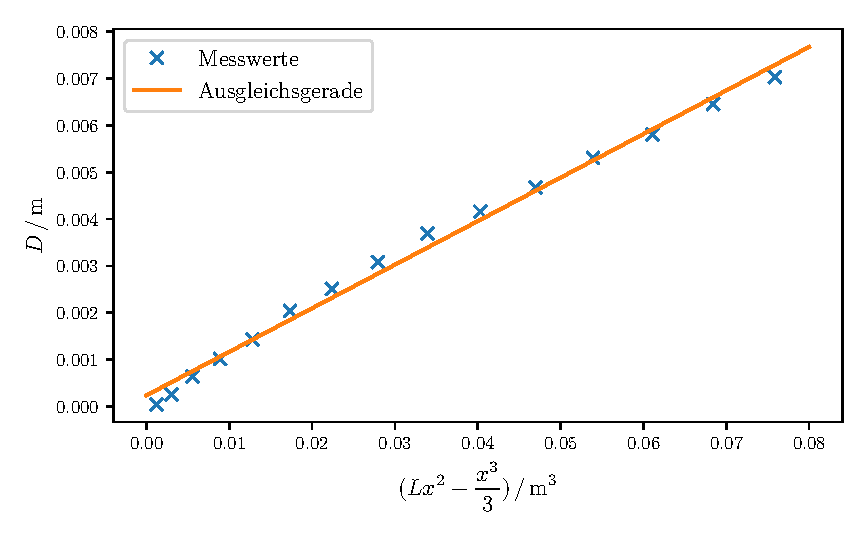
\includegraphics{build/plot2.pdf}
  \caption{Eckiger Stab einseitig eingespannt}
  \label{fig:b}
\end{figure}






\subsection{Runder Stab beidseitig eingespannt}


\begin{table}[H]
  \centering
  
  \csvreader[tabular=c|c|c|c,
  head=false, 
  table head= $x\:/\:\si{\centi\meter}$ & $D_{Ohne Gewicht}\:/\:\si{\milli\meter}$ & $D_{Mit Gewicht}\:/\:\si{\milli\meter}$ & $D_{Differenz}\:/\:\si{\milli\meter}$\\
  \midrule,
  late after line= \\]
  {csvData/tabelle3.csv}{1=\eins, 2=\zwei, 3=\drei, 4=\vier}{$\num{\eins}$ & $\num{\zwei}$ & $\num{\drei}$ & $\num{\vier}$}
  
  \caption{Messwerte des runden Stabes bei beidseitiger Einspannung}
  \label{tab:e}
\end{table}
Auch bei der beidseitigen Einspannung kann der Elastizitätsmodul
durch eine Ausgleichsrechnung bestimmt werden. Hierfür werden
die linke und die Rechte Hälfte des Stabes seperat betrachtet
(siehe Abbildung \ref{fig:c}). Die Steigung der Ausgleichsgeraden auf der linken Seite beträgt

\begin{equation*}
  m=(0,0122 \pm 0,0005)\,\si{\meter\tothe{-2}}
\end{equation*}

\noindent und auf der rechten Seite

\begin{equation*}
  m=(0.01945 \pm 0,00016)\,\si{\meter\tothe{-2}}.
\end{equation*}
\noindent Mit dem entsprechenden Wert $F=11,855 \, \si{\newton}$
für beide Gewichte ergibt sich dann aus dem Zusammenhang

\begin{equation}
  E_{Rund}=\frac{F}{48 \cdot m \cdot I_{Rund}}
\end{equation}

\noindent für $x<L/2$

\begin{equation*}
  E=(99 \pm 4) \cdot 10^9 \,\si{\kilo\gram\per\meter\per\second\squared}
\end{equation*}


\noindent und für $x>L/2$
\begin{equation*}
  E=(62 \pm 6) \cdot 10^9 \,\si{\kilo\gram\per\meter\per\second\squared}.
\end{equation*}

\begin{figure}[H]
  \centering
  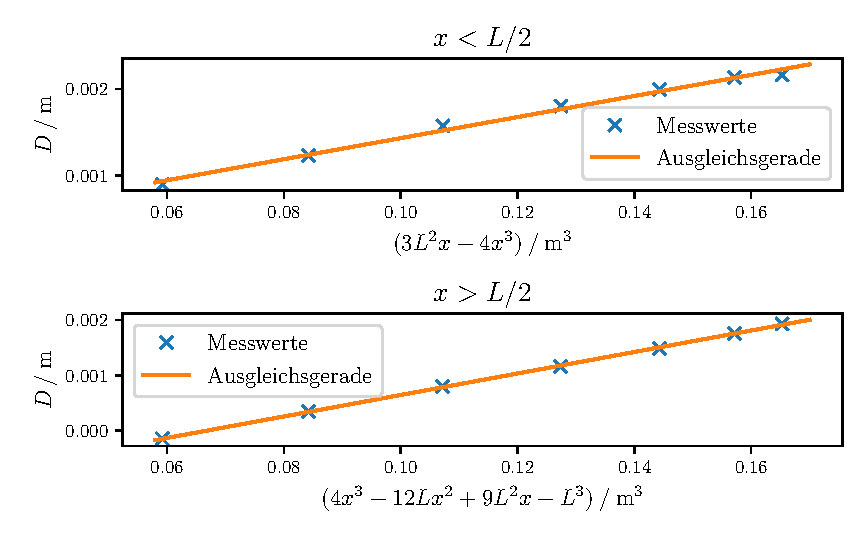
\includegraphics{build/plot3.pdf}
  \caption{Runder Stab beidseitig eingespannt}
  \label{fig:c}
\end{figure}





\subsection{Eckiger Stab beidseitig eingespannt}


\begin{table}[H]
  \centering
  
  \csvreader[tabular=c|c|c|c,
  head=false, 
  table head= $x\:/\:\si{\centi\meter}$ & $D_{Ohne Gewicht}\:/\:\si{\milli\meter}$ & $D_{Mit Gewicht}\:/\:\si{\milli\meter}$ & $D_{Differenz}\:/\:\si{\milli\meter}$\\
  \midrule,
  late after line= \\]
  {csvData/tabelle4.csv}{1=\eins, 2=\zwei, 3=\drei, 4=\vier}{$\num{\eins}$ & $\num{\zwei}$ & $\num{\drei}$ & $\num{\vier}$}
  
  \caption{Messwerte des eckigen Stabes bei beidseitiger Einspannung}
  \label{tab:f}
\end{table}

Die Steigung der Ausgleichsgeraden in Abildung \ref{fig:d}
auf der linken Seite beträgt

\begin{equation*}
  m=(0,0095 \pm 0,0004)\,\si{\meter\tothe{-2}}
\end{equation*}

\noindent und auf der rechten Seite

\begin{equation*}
  m=(0.0089 \pm 0,0006)\,\si{\meter\tothe{-2}}.
\end{equation*}
\noindent Mit dem entsprechenden Wert $F=11,855 \, \si{\newton}$
für beide Gewichte ergibt sich dann aus dem Zusammenhang

\begin{equation}
  E_{Eckig}=\frac{F}{48 \cdot m \cdot I_{Eckig}}
\end{equation}

\noindent für $x<L/2$

\begin{equation*}
  E=(127 \pm 5) \cdot 10^9 \,\si{\kilo\gram\per\meter\per\second\squared}
\end{equation*}


\noindent und für $x>L/2$
\begin{equation*}
  E=(135 \pm 9) \cdot 10^9 \,\si{\kilo\gram\per\meter\per\second\squared}.
\end{equation*}



\begin{figure}[H]
  \centering
  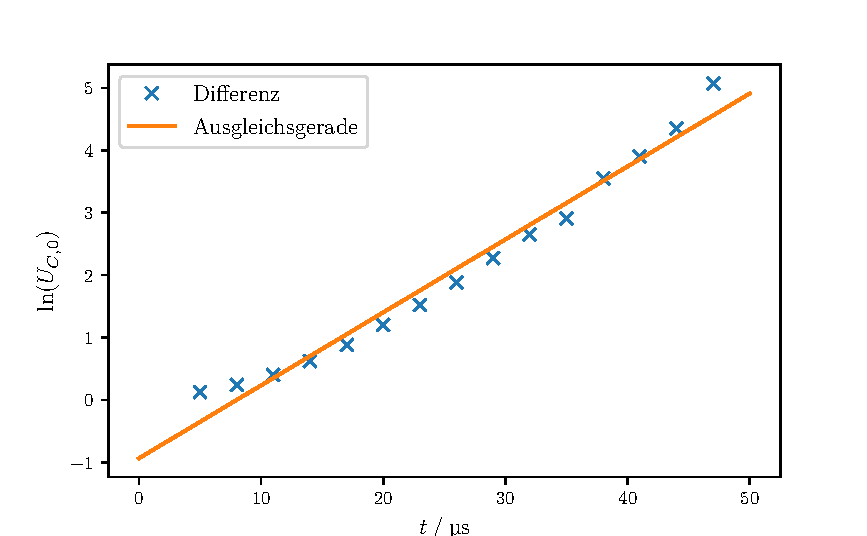
\includegraphics{build/plot4.pdf}
  \caption{Eckiger Stab beidseitig eingespannt}
  \label{fig:d}
\end{figure}




